\documentclass[border=6pt]{standalone}
\usepackage{tikz}
\usetikzlibrary{arrows.meta,automata,positioning}
\begin{document}
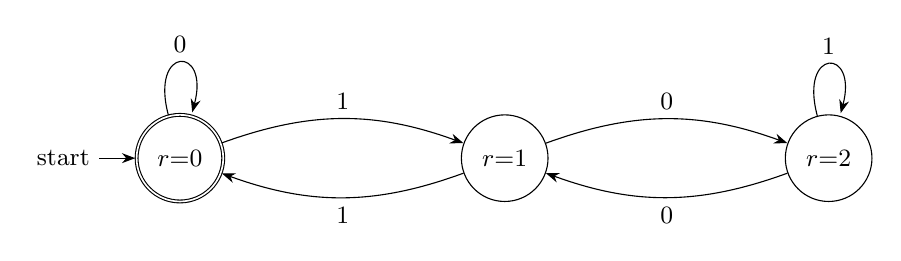
\begin{tikzpicture}[>=Stealth,font=\small,node distance=3cm,auto,
 every state/.style={minimum size=1.1cm}]
\node[state,initial,accepting] (q0) {$r{=}0$};
\node[state,right=of q0] (q1) {$r{=}1$};
\node[state,right=of q1] (q2) {$r{=}2$};
\path[->]
 (q0) edge[loop above] node {0} ()
 (q0) edge[bend left=20] node {1} (q1)
 (q1) edge[bend left=20] node {1} (q0)
 (q1) edge[bend left=20] node {0} (q2)
 (q2) edge[bend left=20] node {0} (q1)
 (q2) edge[loop above] node {1} ();
\end{tikzpicture}
\end{document}
